% TeX source
%
% Author: Tetsuya Ishikawa <tiskw111@gmail.com>
% Date  : January 20, 2020
%%%%%%%%%%%%%%%%%%%%%%%%%%%%%%%%%%%% SOURCE START %%%%%%%%%%%%%%%%%%%%%%%%%%%%%%%%%%%

本文書の目的は,カーネルサポートベクターマシン(以下,K-SVMと略す)を理解することにあります.
職場の同僚や友人から良く受ける質問のひとつに「K-SVMのハイパーパラメータはどのように調整すれば良いか?」
というものがあります.
彼らはグリッドサーチや直感(?!)などでハイパーパラメータを探索・調整しているのですが,
「中身をきちんと理解していれば,手動でちょろっと調整方法することもできるのになぁ」と思うことがあります.
もちろんグリッドサーチが悪いと言っているのでは決してありません.
最終的に性能を出そうとすれば,ある程度の領域に目星を付けた上でグリッドサーチなどの
パラメータ探索手法を使用するのが一般的です.しかしその「目星」を付けられるかどうかは非常に重要です.
さもなければグリッドサーチの探索範囲が爆発し,実時間内に良いハイパーパラメータが探索できなくなってしまいます.
また,SVMはその汎化性能を利用して「ちょっとお試しで」使うことも多いのですが,
そういうときにもハイパーパラメータの目星が付けられないと,そういった使い方もしにくくなります.
ならば同僚に解説文書を読ませてみようかな,と思ったのがこの文書を書くきっかけでした.

本節では,サポートベクターマシン(以下,SVMと略します)について,数式を出さずにラフにお話ししてみましょう.
そもそもSVMとは,与えられた教師付き学習データから2クラスのパターン識別器を構成するための手法です.
ここで強調したいのは,SVMの本質は回帰にある,という点です.
つまり,SVMなんて小難しい名称をしていますが,結局は学習データを曲面で回帰し,
得られた回帰曲線を判別器として利用する,という処理をしているだけに過ぎません.
ちょっと乱暴かもしれませんが,言ってしまえば最小二乗法による点群の回帰とほとんど同じなのです.
ただし,「回帰」ではなく「分類」として高い性能が出るよう,
通常とはやや異なる特殊なやり方で回帰を行う点に,SVMの工夫があるだけです.

具体例でご説明しましょう.
図\ref{fig:example_1}左に示すように,クラスAあるいはBに属する2次元の点群があったとします.
ここでの目的は,図\ref{fig:example_1}右のようにクラスAとBをうまく識別できるような判別曲線を作成することとします.
このような判別曲線を作っておけば,どちらのクラスに分類されるか分からない点が与えられたとき,
この判別曲線を用いて自動的にクラスAかBかを判別できるためです.
\begin{figure}[t]
    \centerline{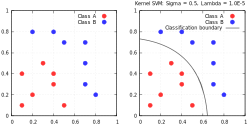
\includegraphics[width=230pt]{figures/example_ksvm_1.pdf}}
    \caption{2クラス分類の例とK-SVMによる判別曲線}
    \label{fig:example_1}
\end{figure}
これを行うために,まずデータの次元を1つ拡大し,3次元にします.
この拡大された3つ目の次元を,ここでは$z$軸と呼ぶことにしましょう.
この$z$軸を何に使用するかというと,クラスを表現するために使用します.
つまり,クラスAに属する点群は$z = +1$に,クラスBに属する点群は$z = -1$に設定します.
このときデータ点群の全体は図\ref{fig:example_2}右のようになります.
\begin{figure}[t]
    \centerline{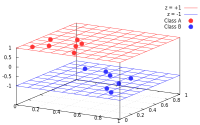
\includegraphics[width=200pt]{figures/example_ksvm_2.pdf}}
    \caption{2クラス分類のデータに$z$軸を追加したところ}
    \label{fig:example_2}
\end{figure}
この拡大されたデータ点群を,曲面で回帰してみましょう.例えば図\ref{fig:example_3}のような曲面が得られたとします.
\begin{figure}[t]
    \centerline{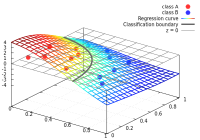
\includegraphics[width=220pt]{figures/example_ksvm_3.pdf}}
    \caption{2クラス分類のデータを曲面で「回帰」したところ}
    \label{fig:example_3}
\end{figure}
先程,クラスAに属する点群は$z = +1$に,クラスBに属する点群は$z = -1$に設定したことを思い出して下さい.
したがって,クラスAの点が多い領域では回帰した曲面も$z = +1$に近くなり,
逆にクラスBが多い領域では回帰曲面は$z = -1$に近づきます.
そこで,この回帰曲面が正の値をとっている領域はクラスAに,
ゼロおよび負の値をとっている領域はクラスBと予測してしまえば良いではないか,と考えるのは自然なことでしょう.
SVMはまさにこれと同じことをしているのです.図\ref{fig:example_2}右の判別曲線は,
図\ref{fig:example_3}の回帰曲面が$z = 0$を交差する場所をプロットしているだけに過ぎません.
これがSVMの基本的なアイディアです.SVMの本質は回帰にある,と言ったのはこのためです.

さらに,回帰曲面としてどの関数を採用するかによってSVMの柔軟性は大きく変化します.
SVMの最も基本的な形態は,回帰曲線に通常の平面(高次元なので正確には超平面)を用いた分類器であり,
これがいわゆる通常のSVMです.本文書ではこれを特に線形SVMと呼ぶことにします.
そして回帰曲面として無限の自由度を持つ局曲面を採用したのがカーネルサポートベクターマシン
(以下,K-SVMと略します)です.図\ref{fig:example_3}は実際にK-SVMで生成した曲面です.

無限の自由度,と聞くと戸惑う読者がおられるかもしれませんが,これは関数をパラメータに持つ回帰関数,という意味です.
例えば,回帰関数のパラメータが$N$次元の実ベクトルであれば,その回帰関数は実$N$次元の自由度を持ち得ますが,
回帰関数のパラメータが関数であれば(すなわち汎関数),その回帰関数は実数では測り切れないほどの自由度を持ち得る,
すなわち無限次元の自由度を持つと言えます.そんな汎関数を回帰関数に定めたのが,K-SVMなのです.

本文書では線形SVMとK-SVMについて解説します.
特にK-SVMの解説では関数空間を全面に押し出した議論を試みています.
読了後に「なーんだ,SVMは(K-SVMも含めて)ただの線形回帰だったのか」と思って頂けたのであれば,
この文書は成功かなと思います.

SVMはVapnik~\textit{et al.}\cite{Vapnik1963}によって,
K-SVMはBoser~\textit{et al.}\cite{Boser1992}によってそれぞれ発表されました.
1900年代の前半には関数解析学がほぼ完成されていたことを考えると,
カーネル法によるSVMの拡張に約30年間もかかったという事実は,個人的にはやや驚きを感じます.
おそらく実ベクトル空間(有限次元)から関数空間(無限次元)という思考の跳躍に時間がかかったのでしょう.
そんな思考の跳躍を体感しながら本文書をお読み頂ければ,著者としてはこの上ない喜びです.

%%%%%%%%%%%%%%%%%%%%%%%%%%%%%%%%%%%% SOURCE FINISH %%%%%%%%%%%%%%%%%%%%%%%%%%%%%%%%%%
% vim: expandtab shiftwidth=4 tabstop=4 filetype=tex
